\section{Morphology}

Morphological operations are yet another set of neighborhood operators however unlike filtering they are designed to modify the shape of objects in binary images specifically. Producing a binary image from a coloured one involves first converting that image to grayscale and then thresholding (Equation \ref{eq:threshold}) its intensity such that pixels are converted to a 1 or 0 depending on whether they lay above or below the threshold (Figure \ref{fig:thresholding}).

\begin{figure}[htbp]
    \centering
    \begin{subfigure}[b]{0.3\textwidth}
        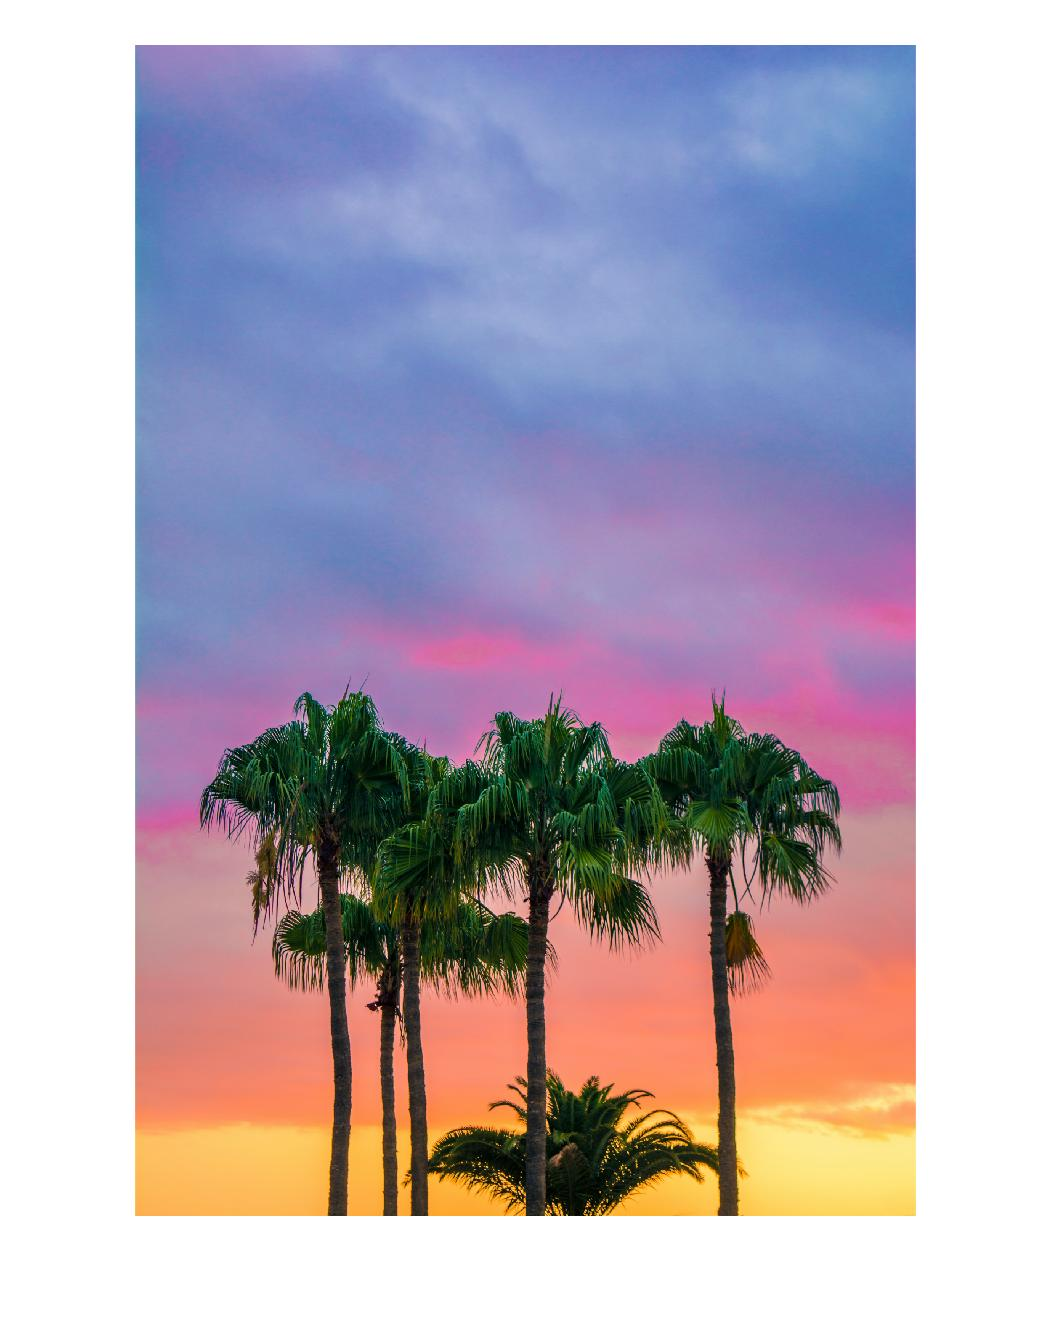
\includegraphics[width=\textwidth]{palms_resized}
        \caption{RGB Image}
        \label{fig:emu_noise}
    \end{subfigure}
    \begin{subfigure}[b]{0.3\textwidth}
        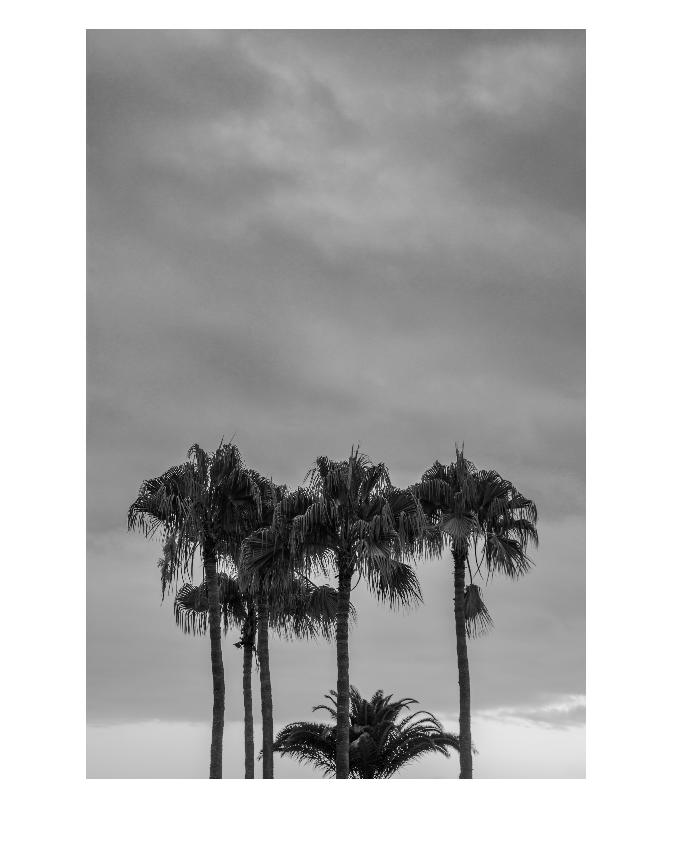
\includegraphics[width=\textwidth]{palms_grayscale}
        \caption{Grayscale Conversion}
        \label{fig:emu_gauss}
    \end{subfigure}
    \begin{subfigure}[b]{0.3\textwidth}
        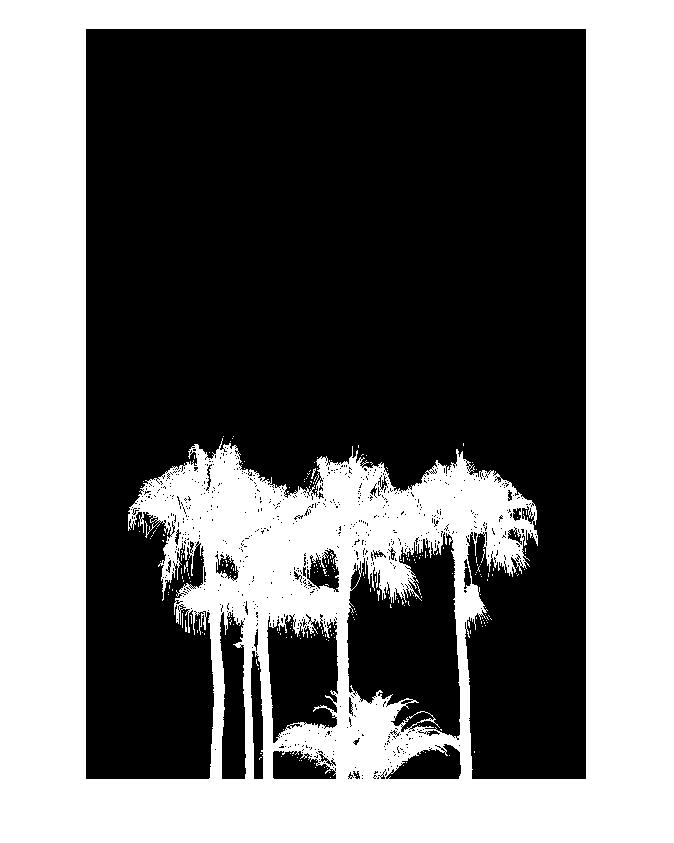
\includegraphics[width=\textwidth]{palms_binary}
        \caption{Binary Thresholding}
        \label{fig:emu_median}
    \end{subfigure}
    \captionsetup{format = hang}
    \caption{Conversion of an RGB image to a binary image. Original image by Adam Birkett}
    \label{fig:thresholding}
\end{figure}